\section{Diagrama de base de datos}

\noindent
Los datos que un sistema recibe, almacena, procesa y muestra son de vital importancia para el correcto funcionamiento del propio sistema o bien, para brindar ciertas tareas al usuario final o, facilitarle otras. Es entonces que el cuidado y el buen almacenamiento de los datos es, de igual forma, sumamente importante. Así, se debe diseñar para cada sistema una estructura que permita almacenar los datos de la forma más conveniente, cubriendo normas dadas que ayudan a que el tratamiento de los datos sea mejor. 
\newline
Para el proyecto ESCOMobile se ha diseñado una base de datos que contempla todas las diferentes entidades consideradas para que éste funcione, teniendo presente, además, las normas referidas, teniendo así, un resultado correcto, mismo que se muestra a continuación:

\begin{figure}[!htpb]
	\hypertarget{fig:baseDatos}{\hspace{1pt}}
	\begin{center}
		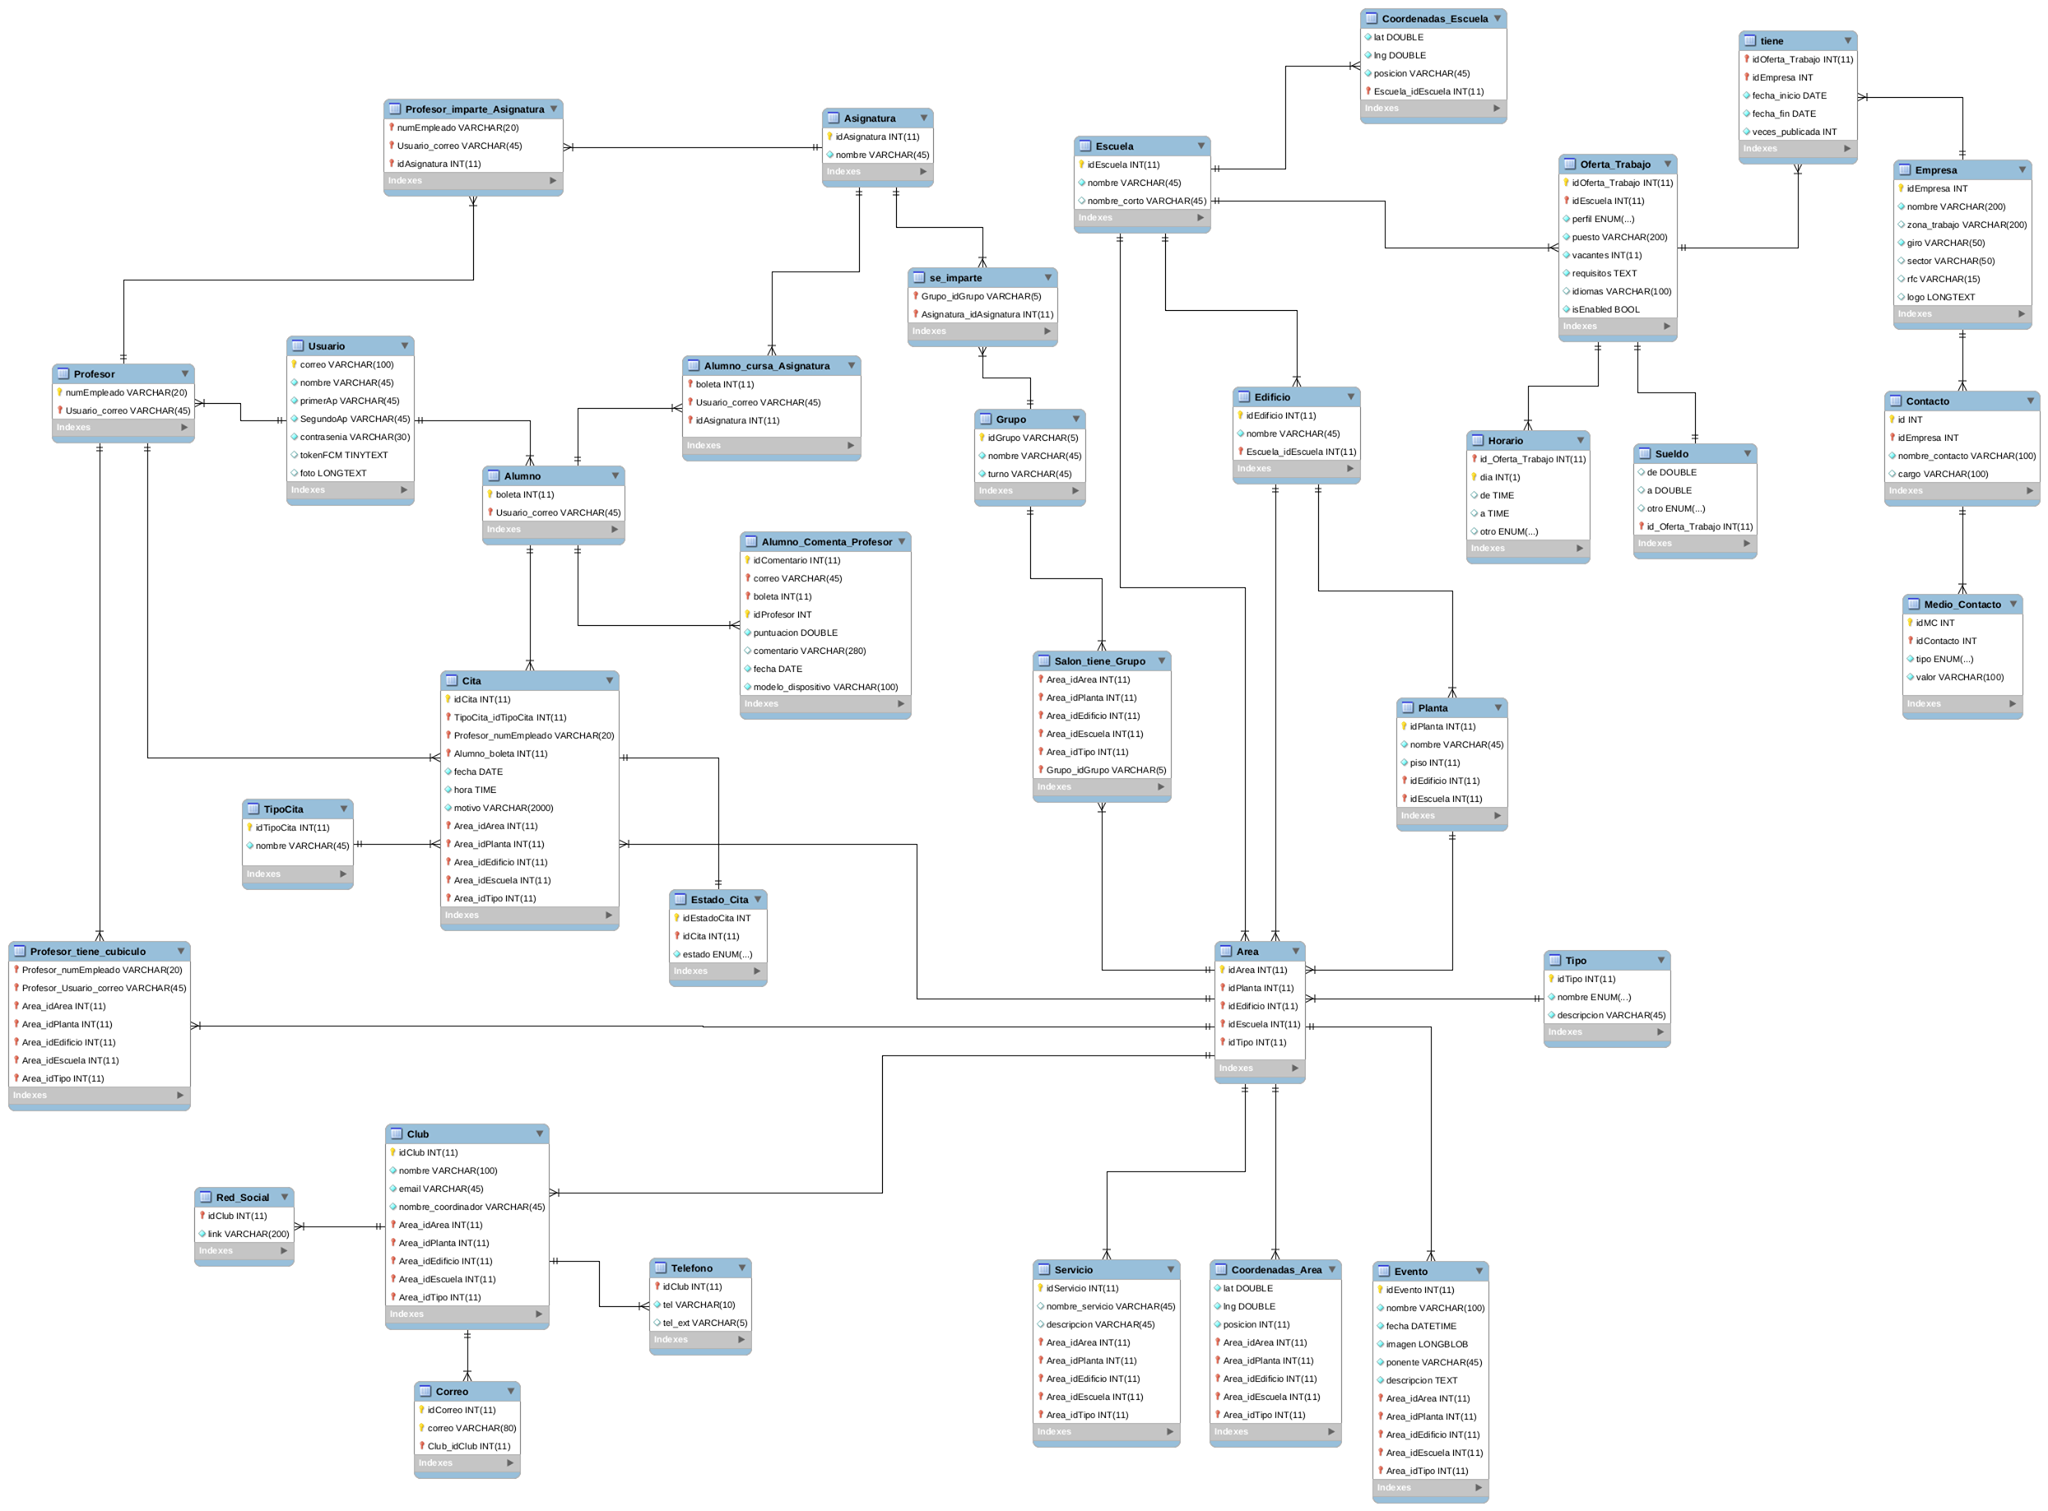
\includegraphics[width=1\textwidth]{images/clases/baseDatos}
		\caption{Diagrama de Base de Datos.}
		\label{fig:baseDatos}
	\end{center}
\end{figure}